
\documentclass[12pt,headinclude,headsepline]{article}
\usepackage{comment}
\usepackage[compact]{titlesec}
\usepackage[margin=0.9in,papersize={8.5in,11in}]{geometry}
\usepackage{times}
\usepackage{hyperref}
\usepackage{subfig}
\usepackage{color}
\usepackage{amsmath}
\usepackage{amssymb}
\usepackage[numbers]{natbib}
\usepackage{graphicx}
%
% Header and Footer
%
\usepackage{fancyhdr}
\pagestyle{fancy}
\lhead{Coupled Aero­Structural­Propulsion Design of an Ultra­Light, Highly Flexible Aircraft}
\chead{}
\rhead{}
\lfoot{}
\rfoot{\thepage}
\cfoot{}
\renewcommand{\headrulewidth}{0.4pt}
\renewcommand{\footrulewidth}{0.4pt}

\newcommand{\f}{\frac}
\newcommand{\p}{\partial}
\newcommand{\ds}{\displaystyle}
\newcommand{\mb}{\mathbf}
\newcommand{\mbs}{\boldsymbol}

\DeclareMathOperator*{\argmin}{arg\,min}
\def\kronecker{\otimes}

\begin{document}

\section{Aeroelastic Modeling}

The modeling and design of slender lightweight flexible structures for
human and electric-powered aircraft requires specialized tools due to
the strongly-coupled multidisciplinary physics that govern these
vehicles. In this project, we will use a tightly integrated
multidisciplinary framework for dynamic and static aeroelastic design
optimization.  For the structural modeling, we will use higher-order
isogeometric analysis for the structures that will provide a robust and
efficient analysis and design capability.

Isogeometric analysis (IGA) techniques are attractive since they
enable CAD-compatible geometry modification while retaining the
advantages of high-order structural analysis. IGA methods utilize the
underlying b-spline basis functions from the geometry model for
displacement interpolation, producing smooth and accurate displacement
and stress solutions. The improved smoothness properties of the stress
distribution from IGA shells smooths the design space for
stress-constrained mass minimization with gradient-based design
optimization.

Integration of aerodynamic, structural, and dynamic aeroelastic design
criteria will be required to achieve a lightweight design that
satisfies all design constraints. We will integrate the IGA analysis
within our structural analysis and design code called the Toolkit for
the Analysis of Composite Structures
(TACS)~\citep{Kennedy:2014:TACS}. TACS is a parallel finite-element
code for large-scale structural analysis and design optimization with
sophisticated gradient evaluation capabilities. TACS is also designed
for multidisciplinary analysis and design optimization of composite
structures, with an existing load and displacement transfer scheme
designed for efficient parallel computations.

\subsection{Nonlinear structural modeling}

In this work, we will utilize a third-order isogeometric shell element
for nonlinear structural analysis and design.  This element balances
the computational costs of analysis and gradient evaluation, with the
superior accuracy of higher-order elements. However, quadratic
b-spline elements are susceptible to both shear and membrane
locking~\citep{Babuska:1992:OLR, Chapelle.Bathe}. Therefore, to
alleviate this locking issue, we utilize a mixed-interpolation of
tensorial (MITC) approach~\citep{Dvorkin:1984:CMB, Bucalem:1993:HOM}.

\begin{figure}[h]
  \centering
  \subfloat[Shell formulation]{
    \label{fig:shell-geometry}
    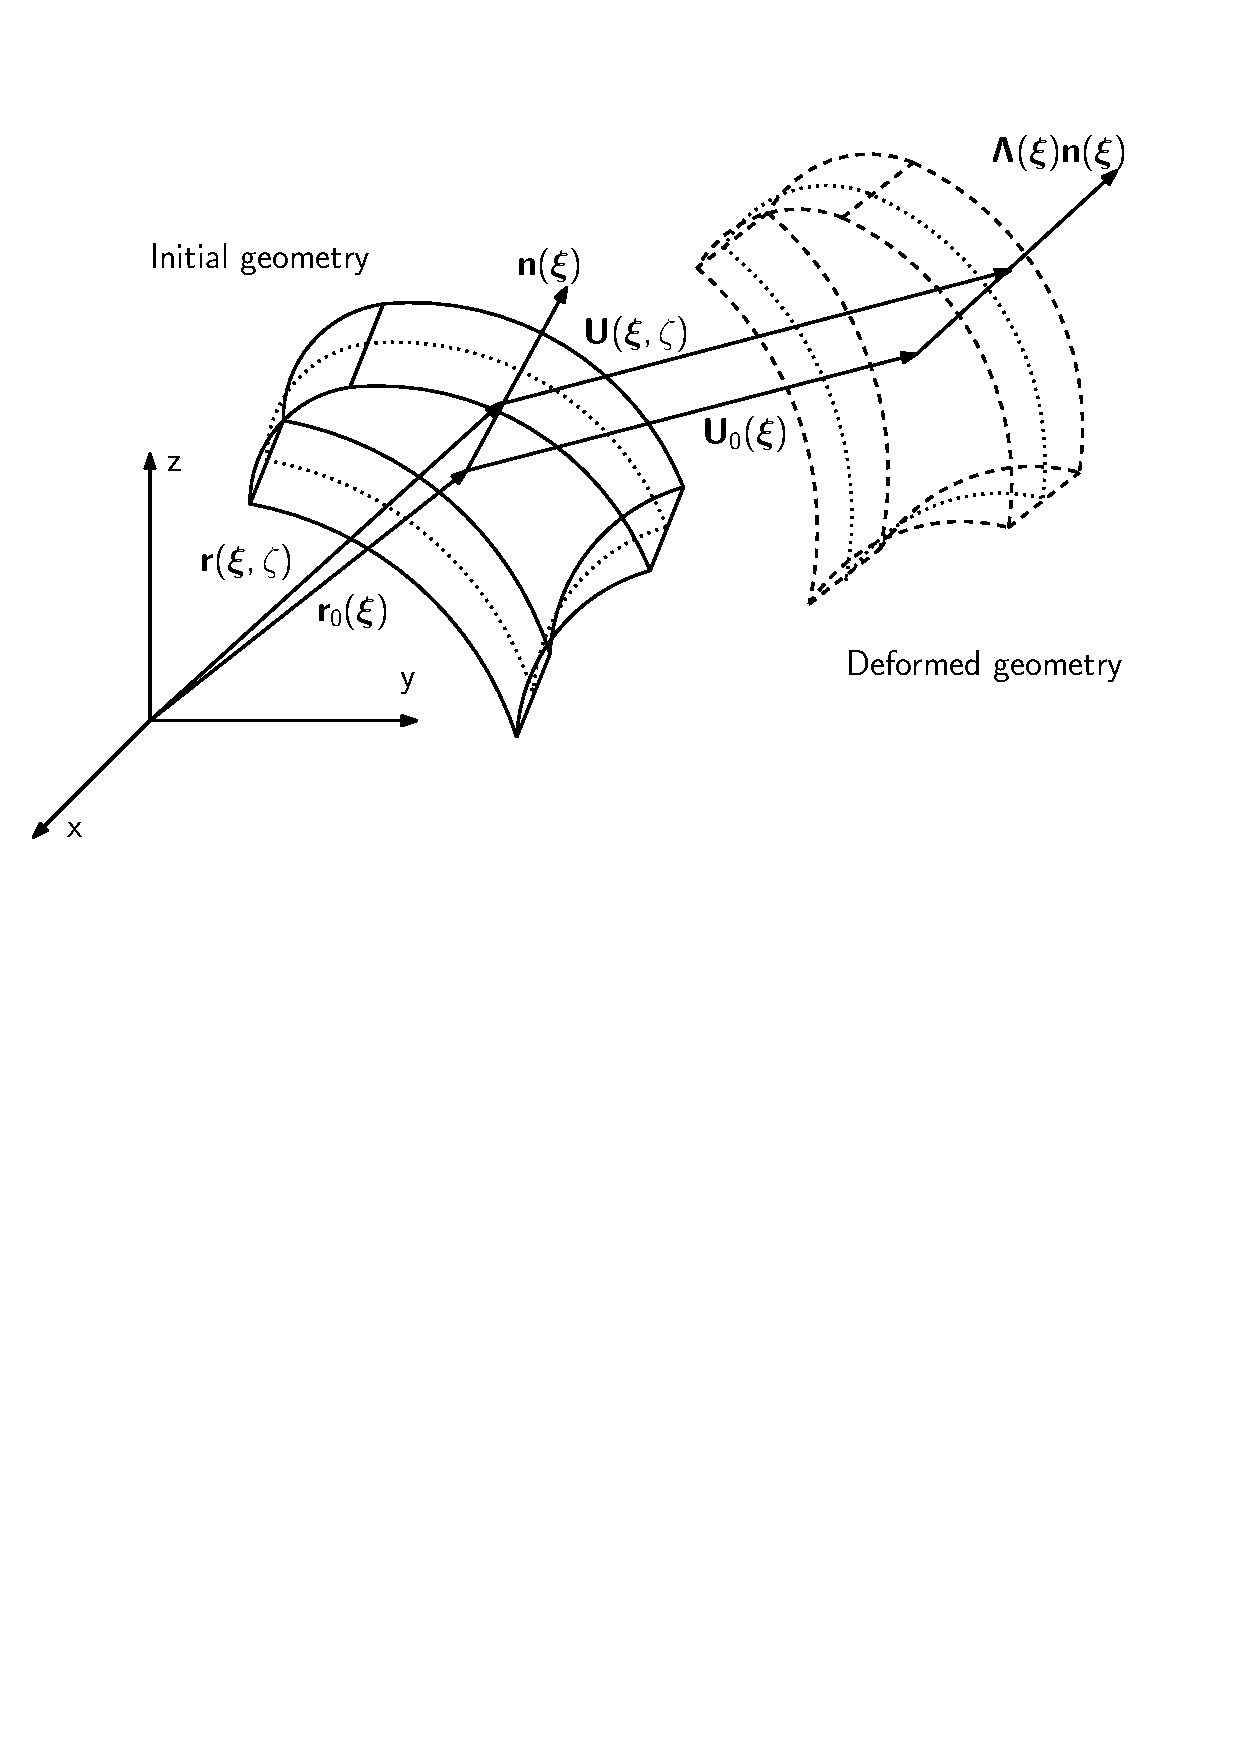
\includegraphics[width=0.4\textwidth]{images/shell_formulation}}
  \subfloat[MITC scheme]{
    \label{fig:mitc-formulation}
    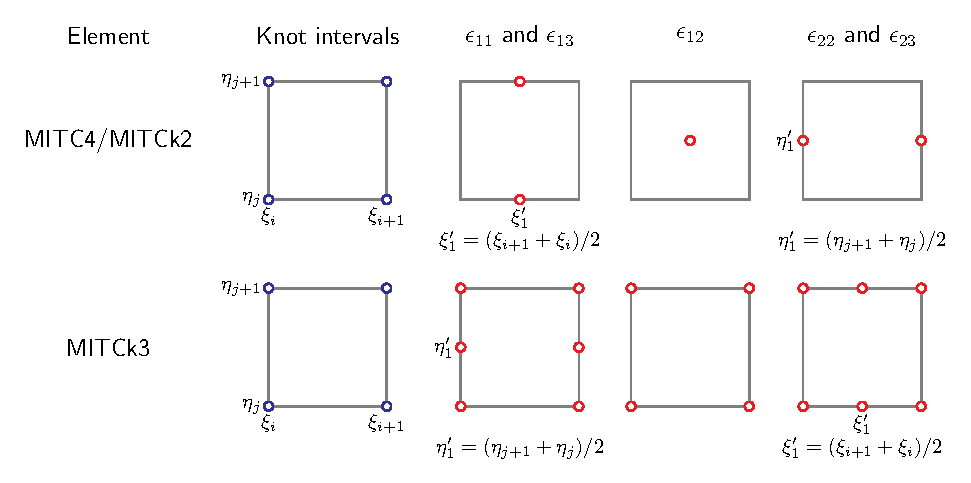
\includegraphics[width=0.6\textwidth]{images/mitc_iga}}
  \caption{The large rotation shell formulation and the b-spline
    compatible MITC scheme.}
  \label{fig:shell-figs}
\end{figure}

The formulation of a general shell element for geometrically nonlinear
analysis is extremely challenging. The elements in TACS use a
degenerated solid approach in which each shell element is formulated
by reducing the full three-dimensional equations of elasticity to the
mid-surface using shell-theory-like assumptions about the distribution
of the displacements through the thickness~\citep{Ahmad:1970:ATS,
  Bathe:1980:GMN, Parisch:1978:GNA, Hughes:1981:NFE}.  The degenerated
solid analysis is mathematically equivalent to a shell theory
formulation under similar same modeling
assumptions~\citep{Buechter:1992:STD}. Following
\citet{Milford:1986:DIF} and \citet{Buechter:1992:STD}, we use an
explicit integration of the strain energy through the thickness,
enabling the direct use of the classical first-order deformation
theory (FSDT) constitutive relationships. The in-plane drilling degree
of freedom is included and a penalization technique is used to ensure
compatibility with the in-plane displacements~\citep{Hughes:1989:DDF,
  Simo:1992:FFE, Fox:1992:DRF}. This formulation facilitates
shell-shell intersections.

The initial, undeformed shell geometry is represented in terms of the
mid-surface vector, $\mb{r}_{0}(\mbs{\xi}) \in \mathbb{R}^{3}$, and
the unit normal, $\mb{n}(\mbs{\xi})$, that are written in terms of the
local shell coordinates $\mbs{\xi}$. The through-thickness coordinate
is given by $\zeta$. The entire shell volume can be expressed as
follows:
%
\begin{equation} 
  \mb{r}(\mbs{\xi}, \zeta) = 
  \mb{r}_{0} + \zeta \mb{n}, 
  \qquad \mbs{\xi} \in \Omega \subset \mathbb{R}^{2}, \qquad.
  \label{eqn:mid-surface}
\end{equation}
Figure~\ref{fig:shell-geometry} illustrates the initial and the deformed
configurations of a shell segment. 

For the shell model, we use kinematic assumptions that are consistent
with a large-displacement, finite-rotation shell. In particular, we
use a director-field representation~\citep{Simo:1989:SRG1}, such that
the normal deforms as, $\mb{d} = \mbs{\Lambda} \mb{n}$, where
$\mbs{\Lambda} \in SO(3)$ is a rotation matrix. The through-thickness
displacement is written in terms follows:
%
\begin{equation*}
  \label{eqn:displacement-field}
  \mb{U}(\mbs{\xi}, \zeta) = \mb{U}_{0} + \zeta (\mbs{\Lambda} - \mb{I}) \mb{n}.
\end{equation*}
where $\mb{U}_{0}$ are the mid-surface displacements and $\mbs{\Lambda}$ is
a rotation matrix.

For the finite-element implementation, we utilize an isogeometric
analysis (IGA) approach. IGA methods have the advantages of
higher-order displacement and stress prediction accuracy. In the IGA
method, the basis functions are b-spline functions which are defined
using the Cox-de~Boor recursion formula as follows~\citep{NURBSbook}:
%
\begin{equation}
  \label{eqn:b-spline-basis}
  \begin{aligned}
    N_{i,p}(u) & = \f{u - u_{i}}{u_{i+p} - u_{i}} N_{i,p-1}(u) + \f{u_{i+p+1} - u}{u_{i+p+1} - u_{i+1}}N_{i+1,p-1}(u) \\
    N_{i,0}(u) & = \left\{ 
      \begin{array}{l} 
        1 \qquad \text{if}\;\; u_{i} \le u < u_{i+1} \\
        0 \qquad \text{otherwise}
      \end{array} \right.
  \end{aligned}
\end{equation}
%
These basis functions are used to both interpolate the
mid-surface~\eqref{eqn:mid-surface} and construct the displacement and
rotation fields~\eqref{eqn:displacement-field}. Since we use
third-order, bi-quadratic b-spline meshes, our formulation is
susceptible to shear and membrane-locking. To alleviate these issues,
we therefore utilize an mixed interpolation of tensorial components
(MITC) approach that utilizes the tying-point scheme shown in
Figure~\ref{fig:mitc-formulation}.  Note that the scheme for
second-order, bi-linear b-spline surfaces degenerates to the classical
MITC4 shell element.

\subsection{Aeroelastic load and displacement transfer}

For this project, our team will develop a coupled aeroelastic design
capability between TACS and $\text{SU}^2$, using existing parallel
load and displacement transfer
techniques~\citep{Kennedy:2014:tacs-tripan}. 

\begin{figure}
  \centering
  \subfloat[Displacement transfer rigid links]{
    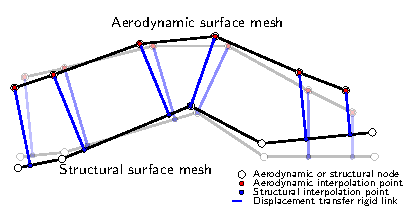
\includegraphics[width=0.5\textwidth]{images/rlink_displaced}
  \label{fig:rigid-link-displacement}}
  \subfloat[Load transfer rigid links]{
    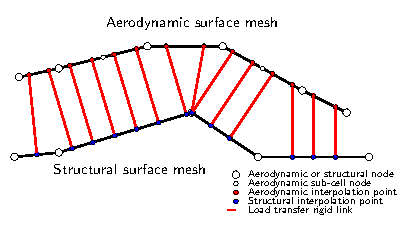
\includegraphics[width=0.5\textwidth]{images/rlink_displacement}
    \label{fig:rigid-link-force}}
  \caption{Load and displacement transfer rigid links for a
    second-order finite-element mesh.}
\end{figure}

This load and displacement transfer technique is a consistent method
based on the method of virtual work. The method works by extrapolating
the displacements from the structural surface to the aerodynamic
surface using both a series of rigid links. These rigid links are
constructed by finding the closest structural surface point to each
aerodynamic mesh location. The rigid links for displacement
extrapolation are illustrated in
Figure~\ref{fig:rigid-link-displacement}.

Next, the aerodynamic surface loads are transferred through a
consistent and conservative technique based on the rigid-link
extrapolation. This integration is computed as follows:
\begin{equation}
  \begin{aligned}
    \delta\, W & = q \int_{S_{A}} \, C_{p} \, \hat{\mb{n}}^{T} \delta\mb{u}_{A} \, \mathrm{d}S \\
    & = q\int_{S_{A}} \, C_{p} \left( \hat{\mb{n}}^{T} \delta \mathbf{u}_{S} -
    \left( \hat{\mb{n}}\times \mb{r}_{SA} \right)^{T} \delta \mbs{\theta}_{S} \right) \, \mathrm{d}S,
  \end{aligned}
  \label{eqn:method-virtual-work}
\end{equation}
where $q$ is the dynamic pressure, $C_{p}$ is the surface pressure
coefficient $\mb{u}_{A}$ and $\mb{u}_{S}$ are the displacements at the
aerodynamic and structural surfaces, $\mbs{\theta}_{S}$ is the
rotation at the structural surface, $\mb{r}_{SA}$ is the rigid-link,
and $\hat{\mb{n}}$ is the normal defined on the deformed aerodynamic
surface.

We approximate the integral~\eqref{eqn:method-virtual-work} by adding the
contributions from each aerodynamic surface cell using a two-part
numerical quadrature rule. First, we split quadrilateral cells based
on a specified characteristic length scale into a series of
subquadrilaterals. The characteristic length scale is selected to
match the length scale of the average finite-element within the
structural model. If any side of the quadrilateral exceeds the
characteristic length scale, we split the cell along that edge into
multiple subcells. Next, on each subcell we use a Gauss quadrature
scheme that matches the order of accuracy required by the underlying
finite-elements. For each quadrature point within each subcell, we
compute a rigid link from the quadrature point to the structural
surface in an analogous manner to the displacement transfer
scheme. This two-level quadrature rule is effective at smoothly
transferring loads to the finite-element mesh even in the presence of
high-aspect-ratio surface cells. Figure~\ref{fig:rigid-link-force}
illustrates the load transfer scheme including the subcell refinement
step.

\subsection{Illustration of the IGA modeling capabilities}

\bibliographystyle{abbrvnat}
\bibliography{../../../papers/biblio/bibfile}

\end{document}
